\documentclass[tikz,border=2pt]{standalone}
\usepackage{amsmath}
\usetikzlibrary{arrows.meta}
\begin{document}
% Three-state bonus-malus chain at fixed lambda: a claim (prob p = 1-e^{-lambda}) sends every state
% to state 1; a claim-free year (prob q = e^{-lambda}) moves 1 -> 2 -> 3 and keeps 3; rows (p,q,0),(p,0,q),(p,0,q).
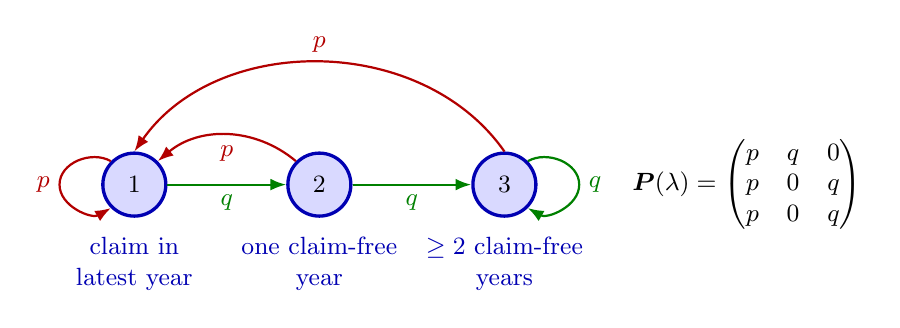
\begin{tikzpicture}[font=\small, >={Latex[length=2mm]},
  st/.style={circle, draw=blue!70!black, very thick, fill=blue!15, minimum size=8mm}]
  \node[st] (s1) at (0,0) {$1$};
  \node[st] (s2) at (2.35,0) {$2$};
  \node[st] (s3) at (4.7,0) {$3$};
  % claim-free moves
  \draw[->, thick, green!50!black] (s1) -- node[below] {$q$} (s2);
  \draw[->, thick, green!50!black] (s2) -- node[below] {$q$} (s3);
  \draw[->, thick, green!50!black] (s3.north east) to[out=30, in=90] (5.65,0) to[out=-90, in=-30] (s3.south east);
  \node[green!50!black, anchor=west] at (5.65,0) {$q$};
  % a claim sends every state back to state 1
  \draw[->, thick, red!70!black] (s1.north west) to[out=150, in=90] (-0.95,0) to[out=-90, in=-150] (s1.south west);
  \node[red!70!black, anchor=east] at (-0.95,0) {$p$};
  \draw[->, thick, red!70!black] (s2.north west) to[bend right=40] node[pos=0.5, below] {$p$} (s1.north east);
  \draw[->, thick, red!70!black] (s3.north) to[out=125, in=55, looseness=1.0] node[pos=0.5, above] {$p$} (s1.north);
  % state descriptions
  \node[blue!70!black, align=center, anchor=north] at (0,-0.55) {claim in\\latest year};
  \node[blue!70!black, align=center, anchor=north] at (2.35,-0.55) {one claim-free\\year};
  \node[blue!70!black, align=center, anchor=north] at (4.7,-0.55) {$\ge2$ claim-free\\years};
  % matrix
  \node[anchor=west] at (6.2,0) {$\boldsymbol{P}(\lambda)=\begin{pmatrix}p&q&0\\p&0&q\\p&0&q\end{pmatrix}$};
\end{tikzpicture}
\end{document}
